\documentclass[handout]{beamer}

\usetheme[progressbar=frametitle]{metropolis}
\metroset{block=fill}

\subtitle{NTIN071 Automata and Grammars}
\author{Jakub Bulín (KTIML MFF UK)}

\date{Spring 2025\\ 
    \vspace{1in} 
    \begin{flushleft}
        \it \footnotesize * Adapted from the Czech-lecture slides by Marta Vomlelová with gratitude. The translation, some modifications, and all errors are mine.
    \end{flushleft}
}

%% packages

\usepackage{amsmath}
\usepackage{amssymb}
\usepackage{amsthm}
\usepackage{cancel}
\usepackage{color}
\usepackage{colortbl}
\usepackage{forest}
\usepackage[utf8x]{inputenc}
\usepackage{multicol}
\usepackage{multirow}

%% colors
\definecolor{Gray}{gray}{0.9}

%% TikZ
\usepackage{tikz}
    \usetikzlibrary{
        automata,
        arrows,
        backgrounds,
        decorations.pathmorphing,
        fit,
        positioning,
        shapes,
        shapes.geometric,
        tikzmark
    } 
    \tikzset{>=stealth',shorten >=1pt,auto,node distance=2cm}
    \tikzset{initial text={}}
    \tikzset{elliptic state/.style={draw,ellipse}}

%% amsthm
\theoremstyle{plain}
    \newtheorem*{algorithm}{Algorithm}    
    \newtheorem*{observation}{Observation}
    \newtheorem*{proposition}{Proposition}

\theoremstyle{remark}
    \newtheorem*{exercise}{Exercise}
    \newtheorem*{remark}{Remark}

%% macros
\DeclareMathOperator{\RegE}{RegE}
\DeclareMathOperator{\RL}{RL}

% Just for Lecture 2
\newcommand{\x}{$\times$}
\newcommand{\nx}{\ }



\title{Lecture 11 -- Turing Machines and grammars, Linear bounded automata and context-sensitive grammars, Intro to computability theory}


\begin{document}


\frame{\titlepage}


\begin{frame}{Recap of Lecture 10}
	
    \begin{itemize}        
        \item Turing machine: two-way infinite tape, read, write, move head
        \item Accept iff in a final state; configurations
        \item TMs with output, computing a function
        \item Recursively enumerable vs. recursive languages (always halt).
        \item Construction tricks: 
        \begin{itemize}
            \item storage in state
            \item multiple tracks (on a single tape)
        \end{itemize}
        \item Variants of TMs: 
        \begin{itemize}
            \item multi-tape (independent heads),
            \item nondeterministic (accept iff some choices lead to final state)
        \end{itemize}  
    \end{itemize}
	
\end{frame}


\section{3.3 Turing Machines and grammars}


\begin{frame}{Chomsky hierarchy: Type 0}

    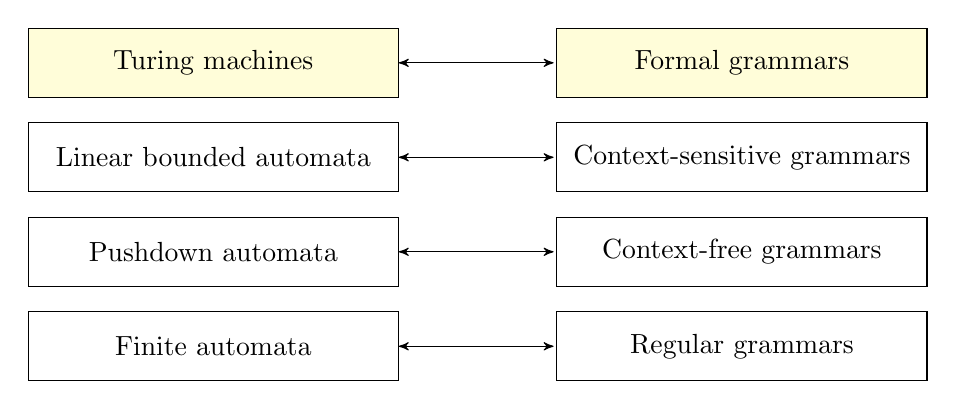
\begin{tikzpicture}[node distance=1.2cm]
        \node[state,rectangle, minimum width =4.7cm][align=center] (fa)      {\alert{Finite automata}};
        \node[state,rectangle, minimum width =4.7cm] (pda) [above of=fa]  {Pushdown automata};
        \node[state,rectangle, minimum width =4.7cm] (la) [above of=pda]  {Linear bounded automata};
        \node[fill=yellow!15!white,state,rectangle, minimum width =4.7cm][align=center] (ts) [above of=la]  {\alert{Turing machines}};
        \node[state,rectangle, minimum width =4.7cm] (rg) [right=2cm of fa]  {Regular grammars};
        \node[state,rectangle, minimum width =4.7cm]  (cfg) [right=2cm of pda]  {\alert{Context-free grammars}};
        \node[state,rectangle, minimum width =4.7cm][align=center]  (cg) [above of=cfg]  {Context-sensitive grammars};
        \node[fill=yellow!15!white,state,rectangle, minimum width =4.7cm] (g0) [above of=cg]  {Formal grammars};
        \path[<->] 
            (fa)  edge node {} (rg)
            (pda)  edge node {} (cfg)
            (la)  edge node {} (cg)
            (ts)  edge node {} (g0)
        ;
    \end{tikzpicture}

    \bigskip

    \begin{theorem}
        A language is recursively enumerable, if and only if it is generated by a Type 0 grammar.
    \end{theorem}
    

\end{frame}


\begin{frame}{Turing machine to grammar}
    
    \begin{itemize}
        \item First generate the relevant portion of the tape and a copy of the input word (nonterminal $\underline{X}$ for each $x\in\Gamma$, in 
        reverse)
        \item Why? TM can rewrite $w$, $G$ must generate it, cannot modify
        \item We have \alert{$wB^n\underline{W}^RQ_0B^m$}, where $B^n$, $B^m$ is sufficient free space        
        \item Then simulate moves (essentially reverse configs+free space)
        \item In a final state erase the simulated tape, keep only $w$
    \end{itemize}
    {\small
    $G=(\{S,C,D,E\}\cup \{\underline{X}\}_{x\in \Gamma}\cup \{Q_i\}_{q_i \in Q},\Sigma,\mathcal P,S)$ where $\mathcal P$ is:
    
    \begin{tabular}{lll}
        (1) 
        & $S\rightarrow DQ_0E$ 
        & simulation starts in initial state 
        \\

        & $D\rightarrow xD\underline{X}\mid E$ 
        & generate input word, reverse copy for simulation
        \\

        & $E\rightarrow BE\mid\epsilon$ 
        & generate sufficient free space for simulation
        \\        
        (2)
        & $\underline{X}P \rightarrow Q\underline{X'} $ 
        & for all $\delta(p,x)=(q,x',R)$ [direction reversed!]
        \\

        & $\underline{X}P \underline{Y}\rightarrow \underline{X'} \underline{Y}Q$ 
        & for all $\delta(p,x)=(q,x',L)$
        \\
        (3) 
        & $P\rightarrow C$ 
        & for all $p\in F$
        \\

        & $C \underline{X}\rightarrow C$,$\underline{X} C\rightarrow C$ 
        & clean the tape
        \\
        
        & $C\rightarrow \epsilon$ 
        & finish, generated $w$
    \end{tabular}
    }

\end{frame}


\begin{frame}{Example: $L=\{a^{2n}\mid n\geq 0\}$}

    $M=(\{q_0,q_1,q_2,q_F\},\{a\},\{a\},\delta,q_0,B,\{q_F\})$ where 
    \begin{align*}
        \delta(q_0,a)&=( q_1,a,R),\\
        \delta(q_1,a)&=(q_0,a,R), \\
        \delta(q_0,B)&=(q_F,B,L)
    \end{align*}
        
    $G=(\{S,C,D,E,Q_0,Q_1,Q_F,\underline{a}\},\{a\},S,\mathcal P_1\cup\mathcal P_2\cup\mathcal P_3)$ \\

    \begin{multicols}{3}
        
        \textbf{Initialize:} $\mathcal P_1$\\
        $S\rightarrow DQ_0E$\\
        $D\rightarrow aD\underline{a}\mid E$\\        
        $E\rightarrow BE\mid\epsilon$

        \newcolumn

        \textbf{Simulate:} $\mathcal P_2$\\
        $\underline{a}Q_0\rightarrow Q_1\underline{a}$\\
        $\underline{a}Q_1\rightarrow Q_0\underline{a}$\\
        $BQ_0\underline{a}\rightarrow B\underline{a}Q_F$
        
        \newcolumn

        \textbf{Cleanup:} $\mathcal P_3$\\
        $Q_F\rightarrow C$\\
        $C\underline{a}\rightarrow C$\\
        $\underline{a}C\rightarrow C$\\
        $BC\rightarrow C$\\
        $C\rightarrow\epsilon$
        
    \end{multicols}
    
    \vspace{-12pt}

    For $w=aa$: initialize \alert{$aaB\underline{a}\underline{a}Q_0$},
     simulate \alert{$aaB\underline{a}Q_F\underline{a}$}, cleanup: \alert{$aa$}

\end{frame}


\begin{frame}{Proof}

    \alert{$L(M)\subseteq L(G)$}

    \begin{itemize}
        \item For $w\in L(M)$ there is a finite accepting sequence of moves
        \item The grammar generates sufficient space
        \item Then we simulate the moves
        \item Finally clean non-input symbols
    \end{itemize}

    \alert{$L(G)\subseteq L(M)$}
    
    \begin{itemize}
        \item Steps in a derivation for $w\in L(G)$ may be in different order
        \item But we can reorder them into the phases (1), (2), (3)
        \item Since we eliminated the underlined symbols, we must have generated the cleaning variable $C$
        \item In order to generate $C$ we must have generated a final state
        \item A final state can only be generated from the initial state by a sequence of simulated moves       
        \hfill\qedsymbol
    \end{itemize}

\end{frame}


\begin{frame}{Grammar to Turing machine}

    \vspace{-1.5cm}
    \alert{Idea:} The TM sequentially generates all possible derivations. (Note: here we do not care about efficiency.)
    \begin{itemize}
        \item code $S\Rightarrow \beta_1\Rightarrow \ldots \Rightarrow  \beta_n=\omega$ as a string $\#S\#\beta_1\#\ldots \#\omega\#$
        \item construct a TM accepting exactly $\#\alpha\#\beta\#$ where $\alpha\Rightarrow\beta$
        \item construct a TM accepting $\#\beta_1\#\ldots\#\beta_k\#$ where $\beta_1\Rightarrow^*\beta_k$
        \item construct a TM generating sequentially all possible strings
        \item check if the string is a valid derivation ending with $\omega$
    \end{itemize}

    \bigskip

    \hspace{1cm}\begin{tikzpicture}[node distance=6cm]
        \tikzstyle{startstop} = [rectangle, rounded corners, minimum width=2cm, minimum height=1cm,text centered, draw=black]
        \tikzstyle{io} = [trapezium, trapezium left angle=70, trapezium right angle=110, minimum width=3cm, minimum height=1cm, text centered, draw=black, fill=blue!30]
        \tikzstyle{process} = [rectangle, minimum width=3cm, minimum height=1cm, text centered, draw=black]
        \tikzstyle{decision} = [diamond,  aspect=2, text width=2cm, minimum height=1cm, text centered, draw=black]        
        \tikzstyle{arrow} = [thick,->,>=stealth]
        \scope[transform canvas={scale=0.65}]
            \node (start) [process] {generate (next) word};
            \node (dec1) [decision, right of=start] {word represents\\a derivation};
            \node (dec2) [decision, right of=dec1] {derivation\\ends with $\omega$};
            \node (s0) [draw=none, below=1.5cm of start] {};
            \node (c0) [draw=none, below=1cm of dec1] {};
            \node (d0) [draw=none, below=1cm of dec2] {};
            \node (d2) [draw=none, right=1cm of dec2] {};
            \draw [arrow] (dec1) -- node {yes} (dec2);
            \draw [arrow] (dec2) -- node {yes} (d2);
            \draw [arrow] (dec1) -- node {no} (c0);
            \draw [arrow] (dec2) -- node {no} (d0);
            \draw [arrow] (s0) -- node {} (start);
            \draw [arrow] (start) -- node {} (dec1);
            %\draw [arrow] (dec2) |- (dec1);
            \path[-]
                            (d0)  edge node {} (c0)
                            (s0)  edge node {} (c0)
            ;
        \endscope
    \end{tikzpicture}

\end{frame}



\section{3.4 Linear bounded automata and context-sensitive grammars}


\begin{frame}{Chomsky hierarchy: Type 1}

    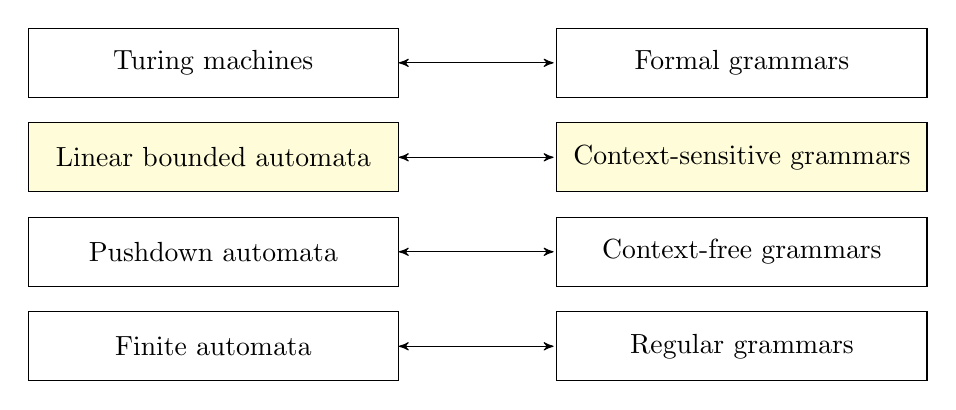
\begin{tikzpicture}[node distance=1.2cm]
        \node[state,rectangle, minimum width =4.7cm][align=center] (fa)      {\alert{Finite automata}};
        \node[state,rectangle, minimum width =4.7cm] (pda) [above of=fa]  {Pushdown automata};
        \node[fill=yellow!15!white,state,rectangle, minimum width =4.7cm] (la) [above of=pda]  {Linear bounded automata};
        \node[state,rectangle, minimum width =4.7cm][align=center] (ts) [above of=la]  {\alert{Turing machines}};
        \node[state,rectangle, minimum width =4.7cm] (rg) [right=2cm of fa]  {Regular grammars};
        \node[state,rectangle, minimum width =4.7cm]  (cfg) [right=2cm of pda]  {\alert{Context-free grammars}};
        \node[fill=yellow!15!white,state,rectangle, minimum width =4.7cm][align=center]  (cg) [above of=cfg]  {Context-sensitive grammars};
        \node[state,rectangle, minimum width =4.7cm] (g0) [above of=cg]  {Formal grammars};
        \path[<->] 
            (fa)  edge node {} (rg)
            (pda)  edge node {} (cfg)
            (la)  edge node {} (cg)
            (ts)  edge node {} (g0)
        ;
    \end{tikzpicture}

    \bigskip

       

\end{frame}


\begin{frame}{Context-sensitive languages}

    \begin{theorem}
        The following are equivalent for a language $L$:
        \begin{enumerate}[(i)]
            \item $L$ is generated by a \alert{context-sensitive} grammar.
            \item $L$ is generated by a \alert{monotone} grammar.
            \item $L$ is recognized by a \alert{Linear Bounded Automaton} (\alert{LBA}).
        \end{enumerate}
    \end{theorem}

    \begin{itemize}
        \item \alert{context-sensitive} grammar: $\alpha_1 A \alpha_2\rightarrow \alpha_1\gamma\alpha_2$ where $A\in V$, $\gamma\in(V\cup T)^+$, $\alpha_1,\alpha_2\in (V\cup T)^*$ ($S\to\epsilon$ if $S$ not in bodies)
        \item \alert{monotone} grammar: $\alpha\to\beta$ where $|\alpha|\leq|\beta|$
        \item \alert{Linear Bounded Automaton} (\alert{LBA}): a nondeterministic TM only using the input portion of the tape [we formalize later]
    \end{itemize}

    \textbf{Note:} Context-sensitive grammars are monotone, $(i)\Rightarrow(ii)$ trivial.\\
    Monotone grammars do not shorten sentential forms in a derivation

\end{frame}


\begin{frame}{Example: $L=\{a^nb^nc^n\mid n\geq 1\} $ is context-sensitive}

    (Recall that $L$ is not context-free.)

    \medskip

    A \alert{monotone} grammar:

    \qquad$S\rightarrow aSBC\mid abC$\hfill{\it right amount of $a,B,C$}\\
    \qquad\alert{$CB\rightarrow BC$}\hfill{\it reorder to $a^nbB^{n-1}C^n$}\\
    \qquad$bB\rightarrow bb$\hfill{\it $B\to b$ only if preceded by $b$}\\
    \qquad$bC\rightarrow bc$\hfill{\it $C\to c$ only if preceded by $b$}\\
    \qquad$cC\rightarrow cc$\hfill{\it\dots or by $c$}

    \bigskip

    The rule $CB\rightarrow BC$ is not context-sensitive. But we can convert it to a chain of context-sensitive rules:

    \qquad$CB\rightarrow XB$, $XB\rightarrow XY$, $XY\rightarrow BY$, $BY\rightarrow BC$

    (Same for any monotone rule, as long as there are no terminals.)
    
\end{frame}


\begin{frame}{From monotone to context-sensitive grammars\hfill $(ii)\Rightarrow(i)$}

    \textbf{Recall:} \alert{separated grammar} means productions of the form $\alpha\rightarrow \beta$ where either $\alpha, \beta\in V^+$ or $\alpha \in V,\beta \in T\cup \{\epsilon\}$

    \begin{lemma}
        Every monotone grammar can be converted to an equivalent context-sensitive grammar.
    \end{lemma}
    \vspace{-6pt}
    \textbf{Proof:}
        First, convert to separated grammar (as for ChNF). This preserves monotonicity, $V_a\to a$ is monotone, context-sensitive.

        Then, convert every production $A_1\ldots A_m\rightarrow B_1\ldots B_n $ ($m\leq n$) to the following chain (using new auxiliary variables $C_i$):
        
        \vspace{-0.9cm}

        \begin{multicols}{2}

            \footnotesize
            
            \begin{align*}
                A_1A_2\ldots A_m & \rightarrow C_1A_2\ldots A_m\\
                C_1A_2\ldots A_m & \rightarrow C_1C_2\ldots A_m\\
                &\ \,\vdots\\
                C_1\ldots C_{m-1}A_m & \rightarrow C_1\ldots C_{m-1} C_m
            \end{align*}

            \newcolumn

            \begin{align*}
                C_1C_2\ldots C_m & \rightarrow B_1C_2\ldots C_m\\
                B_1C_2\ldots C_m & \rightarrow B_1B_2\ldots C_m\\
                &\ \,\vdots\\
                B_1\ldots B_{m-1}C_m & \rightarrow B_1\ldots B_{m-1}B_m\ldots B_n\\                
            \end{align*}
                        
        \end{multicols}

\end{frame}


\end{document}


\section{\sc Chapter 4: Intro to computability theory}


\begin{frame}{Summary of Lecture 11}

    \begin{itemize}        
        \item Recursively enumerable languages are exactly those generated by (Type 0) grammars
        \begin{itemize}
            \item TM to G: simulate moves on a reversed non-terminal copy of $\omega$, generate sufficient space, cleanup if accepting state
            \item G to TM: generate all strings, check if any of them represents a valid derivation of $\omega$ (sentential forms separated by $\#$)
        \end{itemize}   
        \item Context-sensitive languages    
    \end{itemize}
    
\end{frame}


\section*{Linear Bounded Automata}


\begin{frame}{Linear Bounded Automaton}

    We need an automaton counterpart of context grammar:

    \begin{definition}
    \emph{Linear bounded automaton (LBA)} is a *nondeterministic* TM where the tape contains special symbols for left ($\underline{l}$) and right ($\underline{r}$) end. Those symbols cannot be rewritten and the head cannot move to the left of $\underline{l}$ or to the right of $\underline{r}$. 

    A word $w$ is \emph{accepted} by the LBA, if $q_0\underline{l}w\underline{r}\vdash^*\alpha p\beta$ for some $p\in F$
    \end{definition}
    \begin{itemize}
        \item The space for the computation is given by the input word and the automaton cannot exceed its length during the computation
        \item This is not a problem for context (and for monotone) grammars: no sentential form in the derivation can be longer than $w$.
        \item Nondeterminisim is crucial!
    \end{itemize}

\end{frame}


\begin{frame}{Context-sensitive grammar to LBA}

    \begin{theorem}
    Every context language is accepted by some LBA.
    \end{theorem}
    \begin{proof}
    We simulate the derivation of the grammar on the LBA.
    \begin{itemize}
        \item use a two-track tape
        \item first track: $w$ 
        \begin{itemize}
            \item read-only, i.e., not changed during the computation
            \item at the end, compare with 2nd track 
        \end{itemize}
        \item second track: the sentential form 
            \begin{itemize}
                \item at the beginning: $S$ in the first position, the rest is blank
                \item at the end: $w$
            \end{itemize}
    \end{itemize}
    \begin{center}
    \begin{tabular}{|c| c c |c|}
    \hline
    \multirow{2}{*}{\underline{l}} & \multicolumn{2}{c|}{w}& \multirow{2}{*}{\underline{r}}\\ \cline{2-3}
    & \multicolumn{1}{c|}{S}& \hspace{2cm} &\\\hline
    \end{tabular}
    \end{center}

    One step of the derivation: applying the rule $\alpha X \beta \rightarrow \alpha \gamma \beta$

    \begin{center}
    \begin{tabular}{c c c  c c c}
    \cline{1-5}
    \multicolumn{1}{|c|}{u} & $\alpha$ & \multicolumn{1}{|c|}{X} & $\beta$& \multicolumn{1}{|c|}{v} &\\ \cline{1-5}
    \vspace{0.005cm}\\ \cline{1-6}
    \multicolumn{1}{|c|}{u} & $\alpha$ & \multicolumn{2}{|c|}{$\gamma$} & $\beta$& \multicolumn{1}{|c|}{v} \\ \cline{1-6}
    \end{tabular}
    \end{center}

    \begin{itemize}
        \item Rewrite the sentential form in the 2nd track using production rules of $G$
        \item Nondeterministically choose the part to be rewritten and the rule to be used
        \item Rewrite using the chosen rule (move the rest of the track to the right)
        \item If there are only terminals, compare with the 1st track, accept if they match
    \end{itemize}
    \end{proof}

\end{frame}


\begin{frame}{LBA to context-sensitive grammar}
    
    \begin{theorem}
    LBA accept only context languages.
    \end{theorem}
    \begin{proof}
    We will construct a monotone grammar.
    \begin{itemize}
        \item the grammar cannot generate any `extra' symbols
        \item we hide the computation in `two-track' variables
        \item generate word of the form $$(a_0,\left[q_0,\underline{l},a_0\right]),(a_1,a_1),\ldots,(a_n,\left[a_n,\underline{r}\right]) $$
    %	\end{itemize}

    \medskip
    \begin{center}
    \begin{tabular}{|c c c|}
    \hline
    \multicolumn{3}{|c|}{w} \\ \cline{1-3}
    \multicolumn{1}{|c|}{$q_0,\underline{l},a_0$}& \hspace{2cm} &\multicolumn{1}{|c|}{$a_n,\underline{r}$}\\\hline
    \end{tabular}
    \end{center}

    \bigskip
    \item simulate the computation of the LBA in the 2nd track (as we did for TMs)
    \begin{itemize}
        \item for $\delta(p,x)=(q,x',R)$:  $P\underline{X}\underline{Y}\rightarrow \underline{X'}Q\underline{Y}$ 
        \item for $\delta(p,x)=(q,x',L)$:  $\underline{Y}P\underline{X}\rightarrow Q\underline{Y}\underline{X'} $ 
    \end{itemize}
    \item if the state is accepting, `erase' the 2nd track
    \item special production for accepting $\epsilon$ (if $\epsilon \in L$)
    \end{itemize}
    \end{proof}

\end{frame}


\end{document}

